\documentclass[10pt]{beamer}
\usepackage[utf8]{inputenc}
\usetheme[progressbar=frametitle]{metropolis}
\usepackage{booktabs}
\usepackage[scale=2]{ccicons}
\usepackage{pgfplots}
\usepgfplotslibrary{dateplot}
\usepackage{xspace}
\newcommand{\themename}{\textbf{\textsc{metropolis}}\xspace}
\graphicspath{{./Bilder/}}

\title{Spooks}
\subtitle{Skummelt pek og ondskapsfullt klikk \\ (Working title)}
\date{\today}
\author{Mats, Malin, Hans Ivar, Eirik og Ole}
\institute{}

\begin{document}
	
	\maketitle
	
	\begin{frame}{Table of contents}
		\setbeamertemplate{section in toc}[sections numbered]
		\tableofcontents[hideallsubsections]
	\end{frame}
	
	\section{Introduksjon}
	
	\begin{frame}[fragile]{Introduksjon}
		
	  Ideen:

          \begin{itemize}
          \item Skrekkbasert pek-og-klikk spill
          \item Løs gåter for å åpne nye rom
          \item Hvert 5-minutt blir spillinstansen reversert til siste checkpoint
          \item Rendret i 2.5d
          \end{itemize}

          
	\end{frame}
	
	\begin{frame}[fragile]{Sections}
		\begin{itemize}
			\item Målgruppe 12+
			\item {Spilletid: 5-minutt per runde, total spilletid avhenger av hvor lang tid en bruker per runde.}
			\item {En spiller, mot datamaskin}
			\item {Mulig å lagre (helst)}
			\item {Din karakter kan ikke dø, men tidspress og ulike utfordringer kan sørge for at du ``taper''}
			\item {Spilleren må finne og kombinere ulike gjenstander for å løse oppgavene i spillet}
			\item {Når tiden går ut vil spilleren miste alle gjenstander som er plukket opp, men fremgang i spillet vil ikke gå tapt. Spilleren må da være taktisk når det kommer til hvilke gjenstander en plukker med seg for hver runde.}
		\end{itemize}
	\end{frame}
	
	\section{Bruksmønster}
	
	\begin{frame}{Blocks}

          Tekniske alternativer:
		
		\begin{columns}[T,onlytextwidth]
			\column{0.5 \textwidth}
			\begin{block}{Engine}
			  Unity
              JMonkeyEngine
              eller lignende.
			\end{block}
			
			\begin{block}{Platform}
				Windows, Mac, Linux
			\end{block}
			
			\begin{block}{2.5d}
			  Rendret i 3d, men spilleren opplever spillet i 2d.
              Dette vil gjøre det lettere med tanke på lys/dybte-effekter
			\end{block}
				
		\end{columns}

	\end{frame}
	
	\section{Illustrasjoner}
	
	\begin{frame}{Figures}
		
	  \fbox{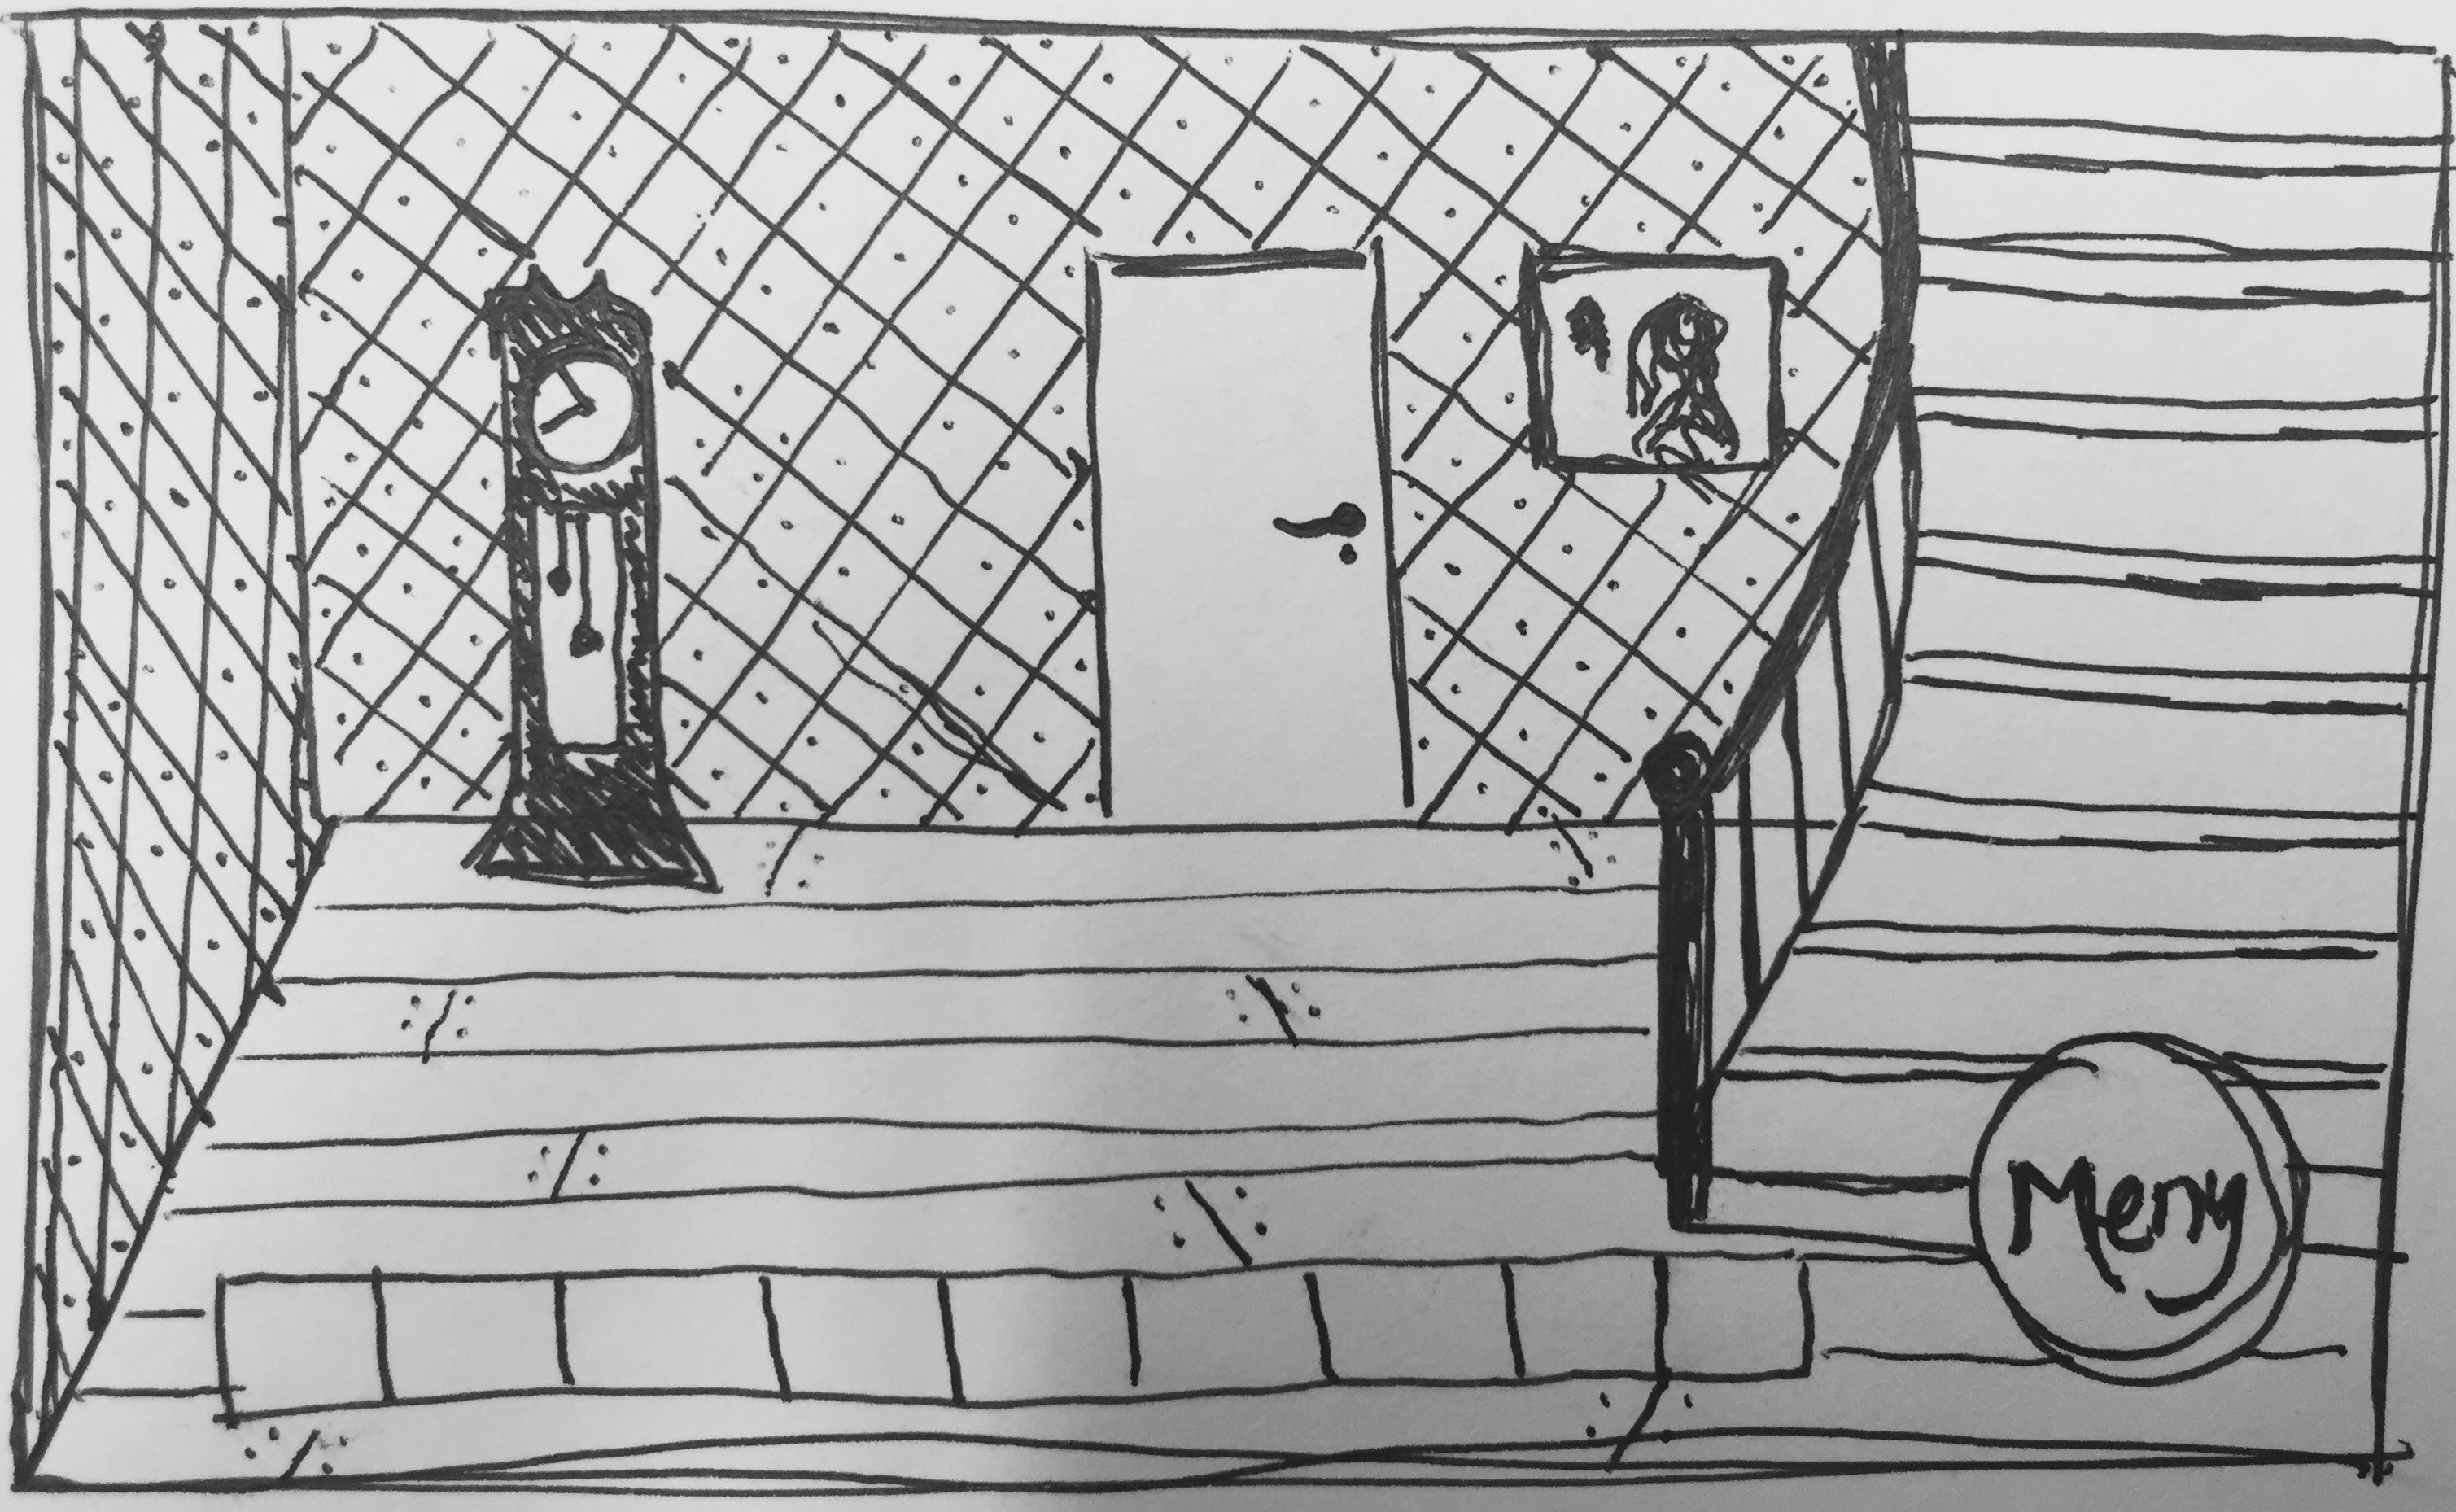
\includegraphics[width=1.02\textwidth]{bilde1.jpg}}
   	  
	\end{frame}
	
	\begin{frame}{Figures}
		
	  \fbox{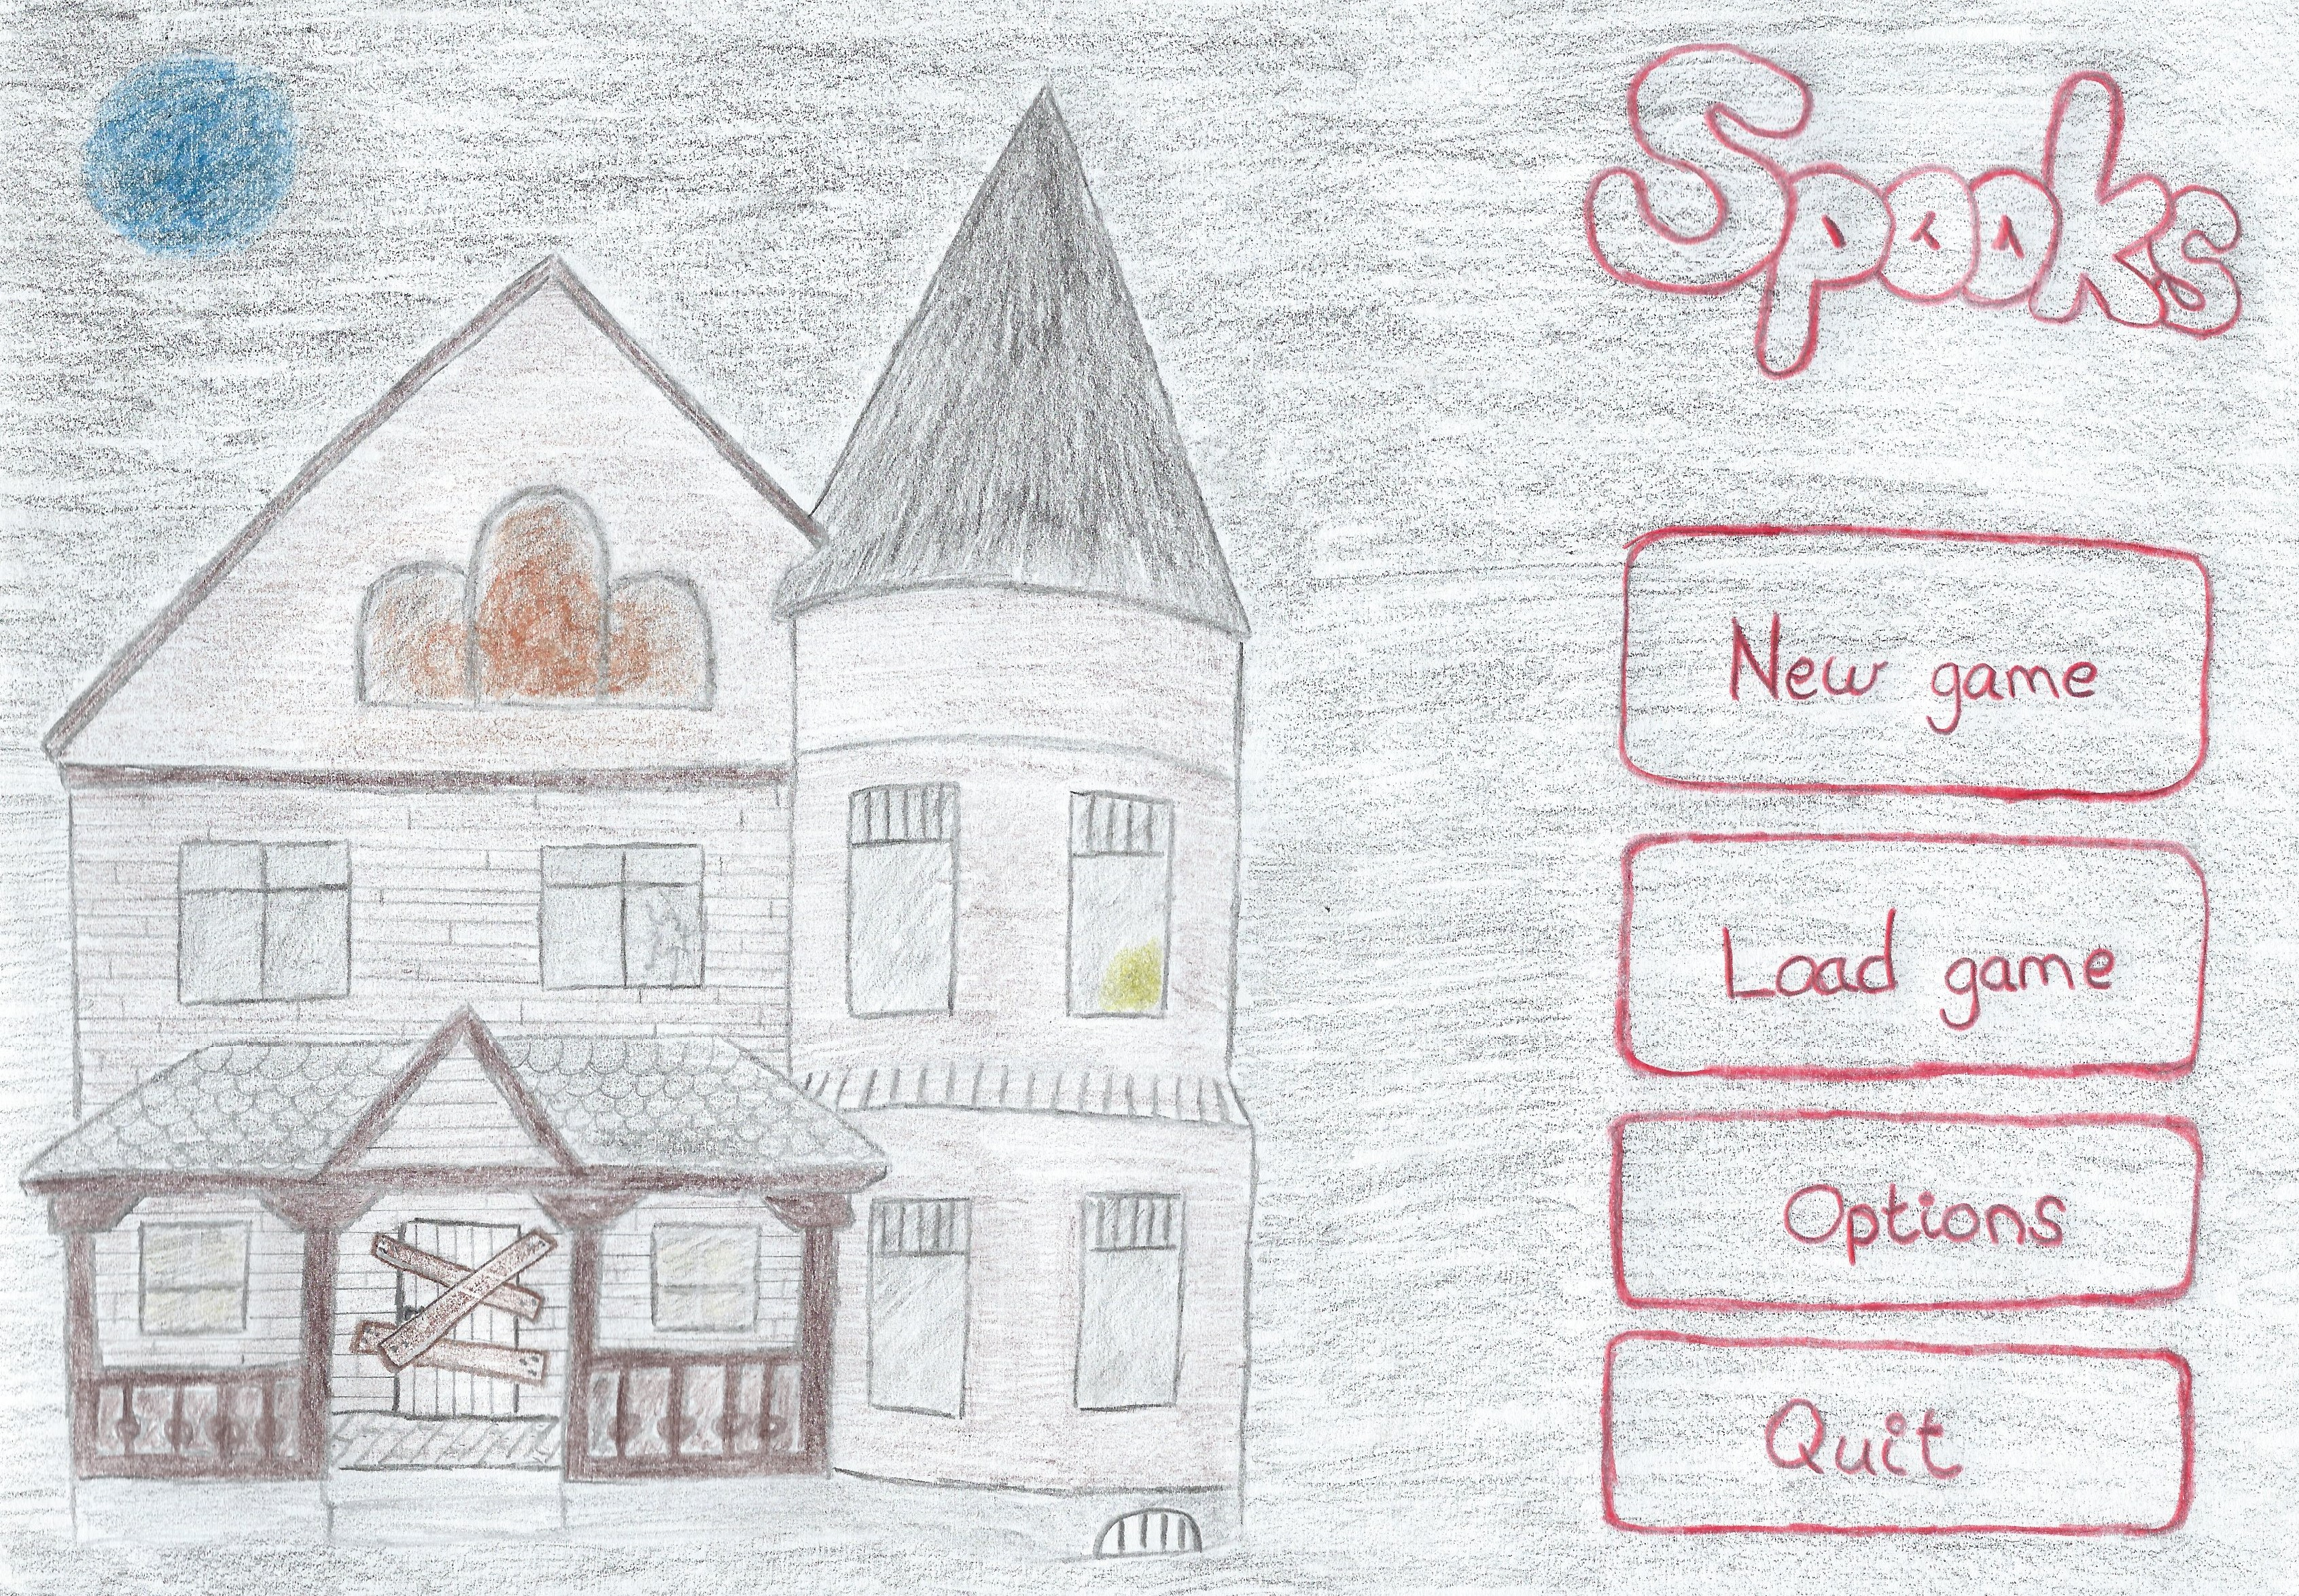
\includegraphics[width=1.02\textwidth]{bilde2.jpg}}
   	  
	\end{frame}

        \begin{frame}{Figures}
		
	  \fbox{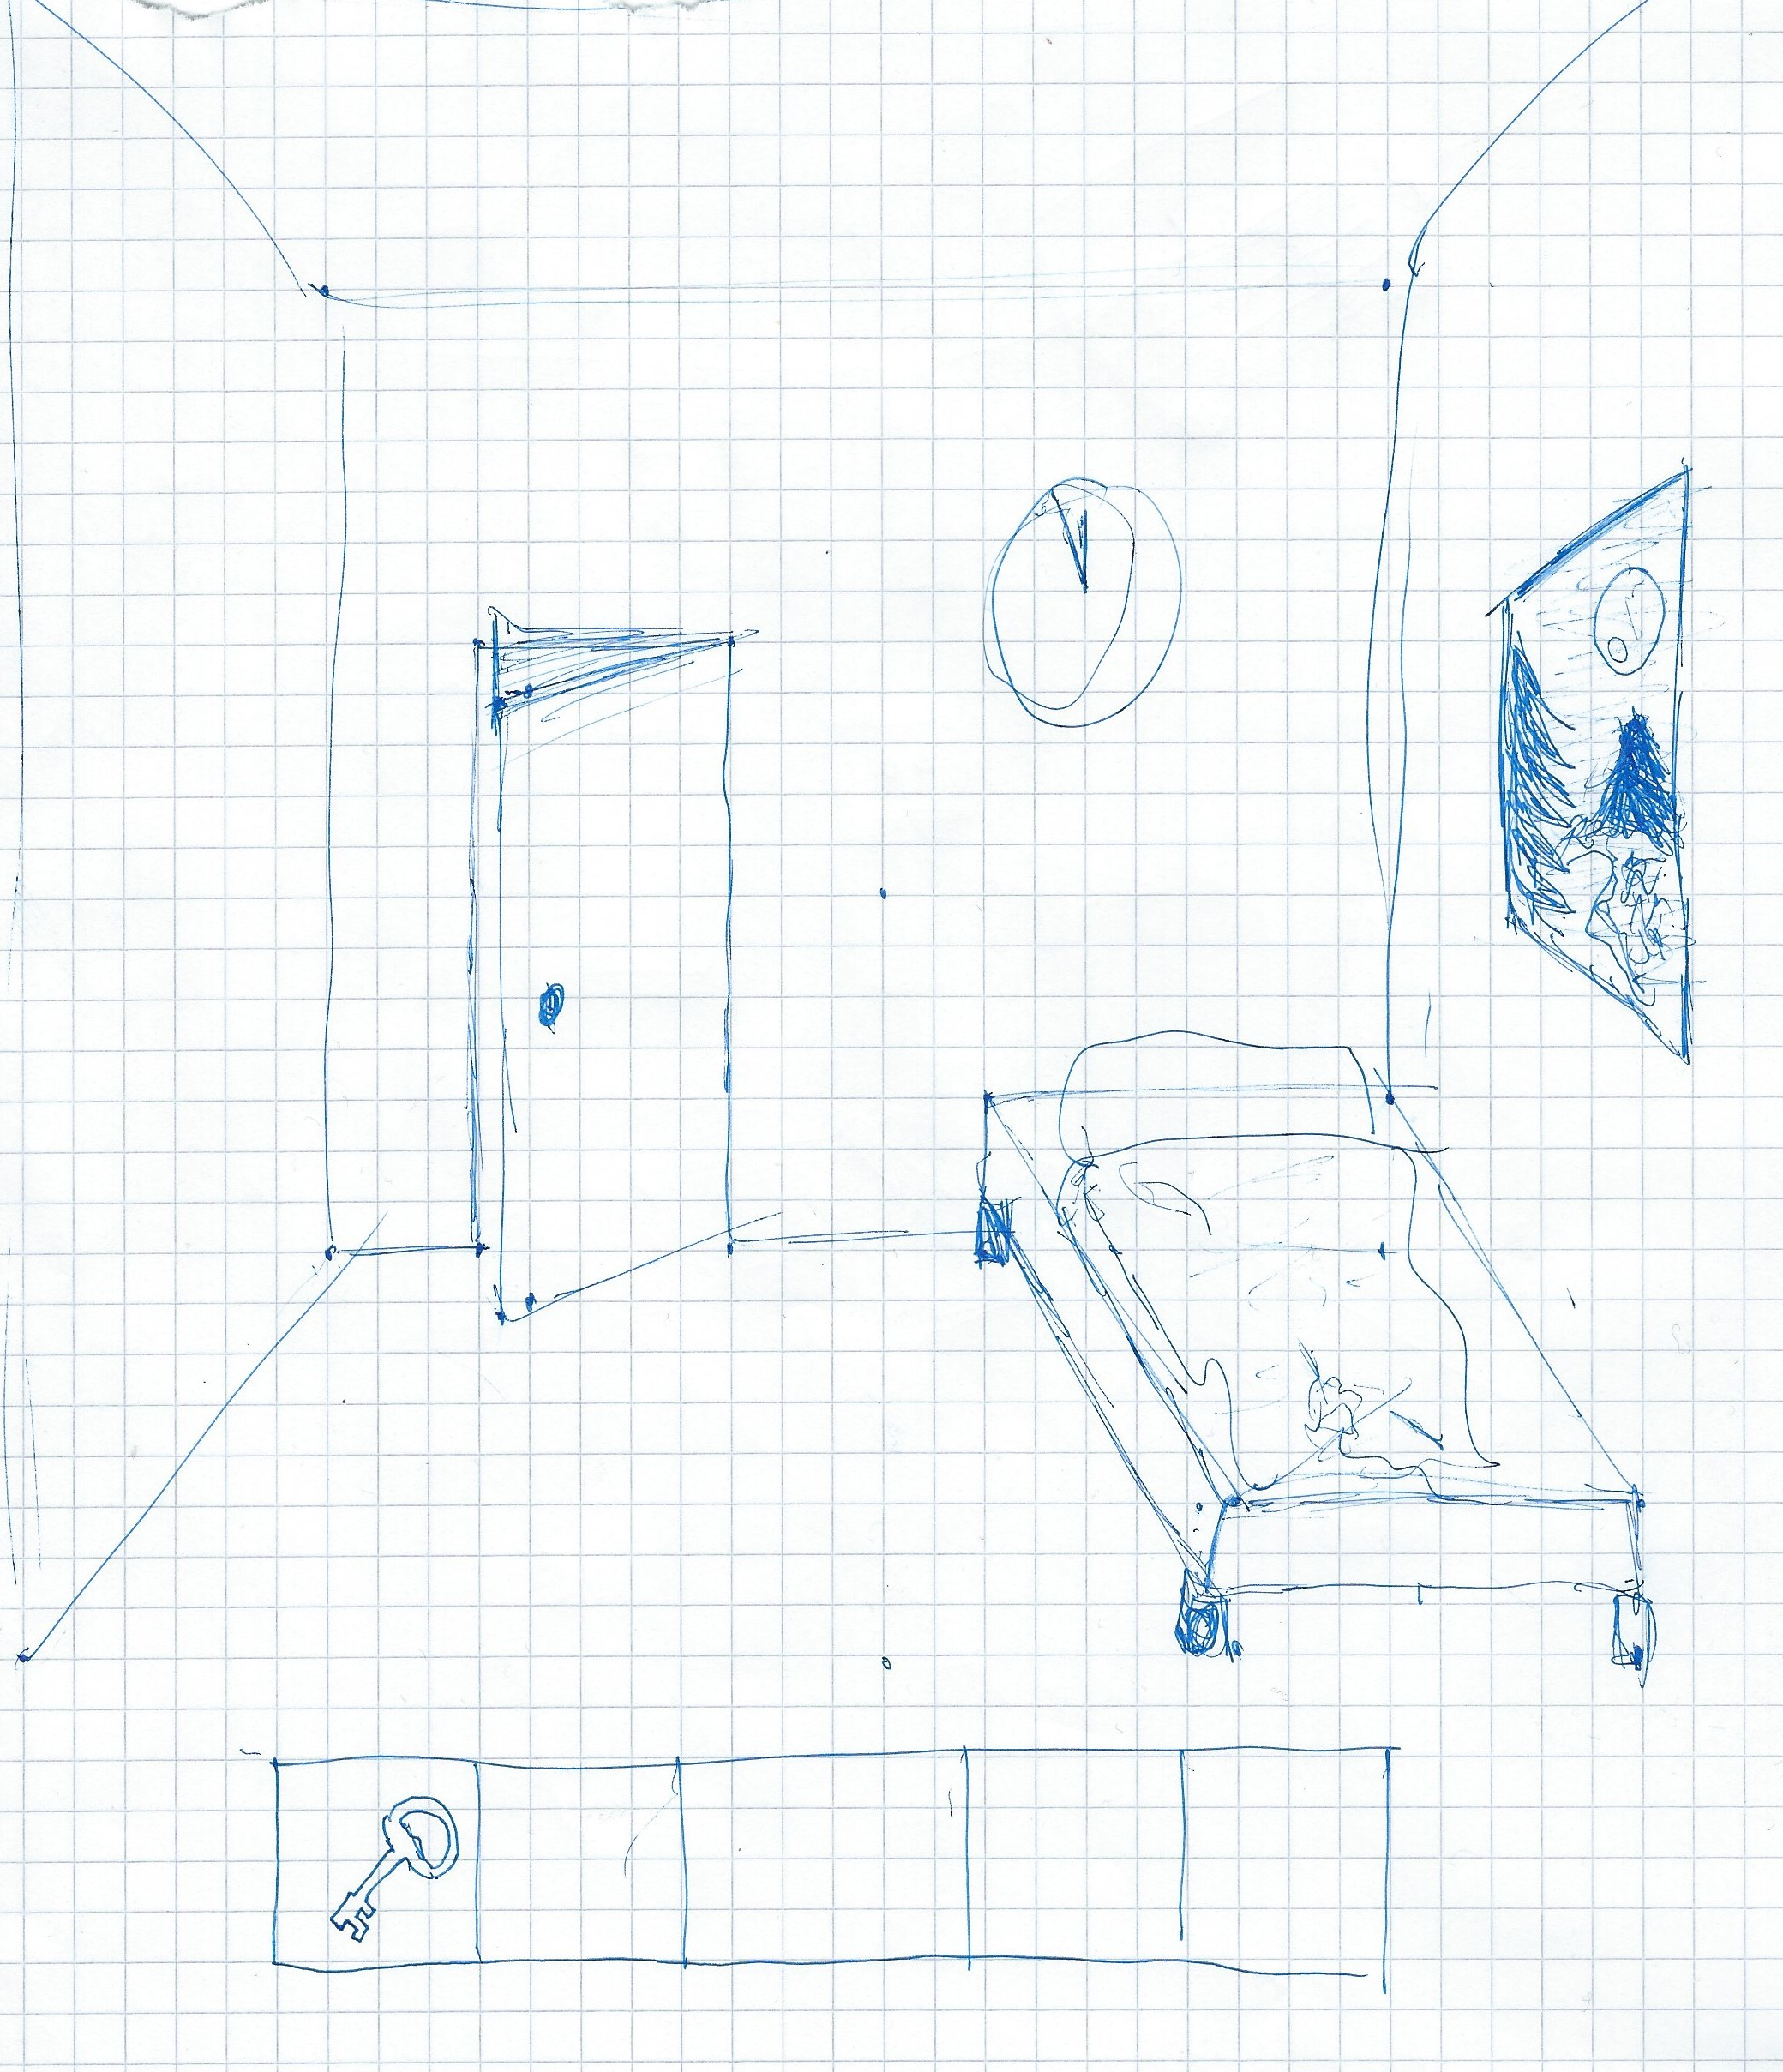
\includegraphics[width=1.02\textwidth]{bilde3.jpg}}
   	  
	\end{frame}
	
	\section{Gjennomføring}
	
	\begin{frame}{Forslag}
		
	\end{frame}
	
	\begin{frame}[standout]
		Spooks
	\end{frame}
	
\end{document}
